\clearpage
\subsection{Server}

L'architettura della componente server si articola in una 3-layer architecture, in cui si identificano i seguenti layer:
\begin{itemize}
	\item communication layer;
	\item business layer;
	\item persistence layer.
\end{itemize}

\begin{figure}[H]
	\centering
	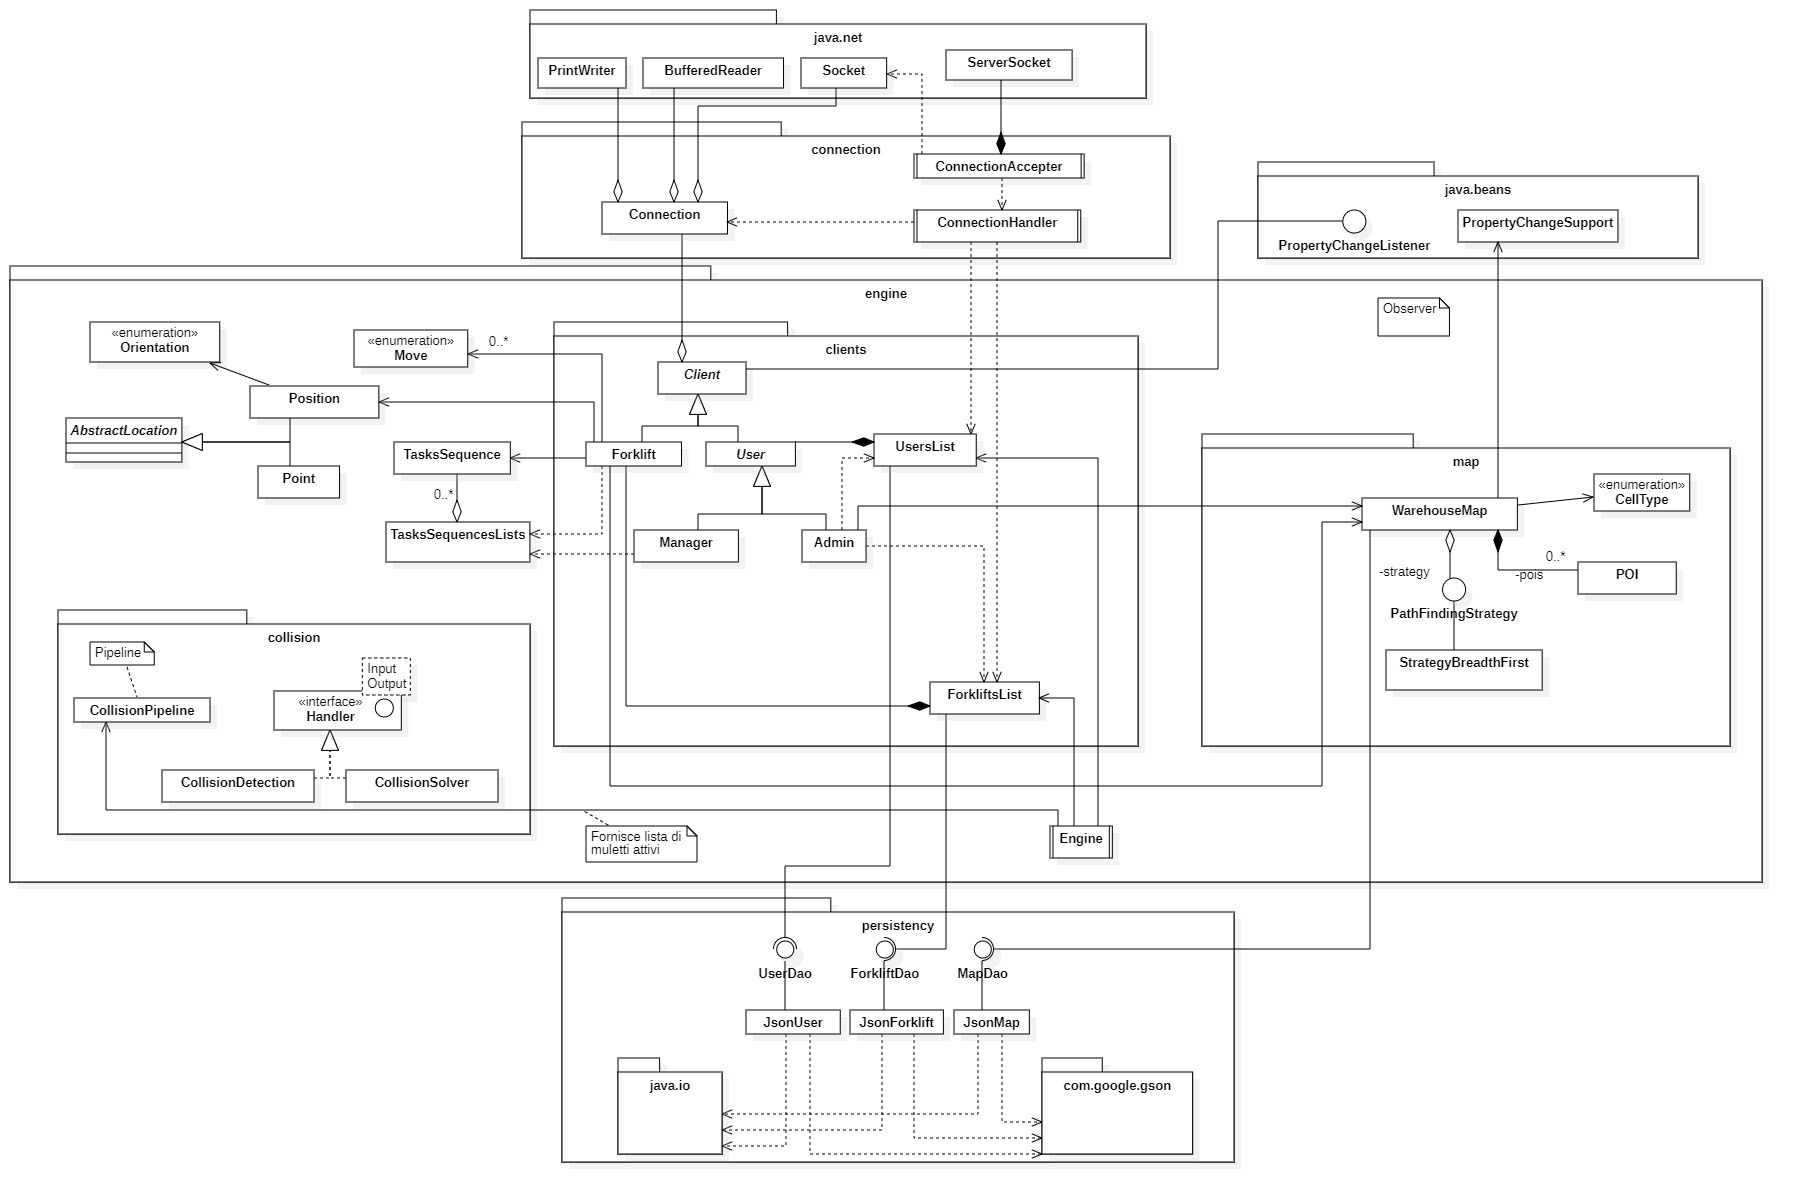
\includegraphics[scale=0.22]{res/diagrams/server/server_complessivo_minimal.jpg}
	\caption{Visione complessiva dell'architettura del server}
\end{figure}

Le sezioni che seguono illustrano la struttura di ogni layer.

\clearpage
\subsubsection{Communication layer}
\label{communication-layer}

\begin{figure}[H]
	\centering
	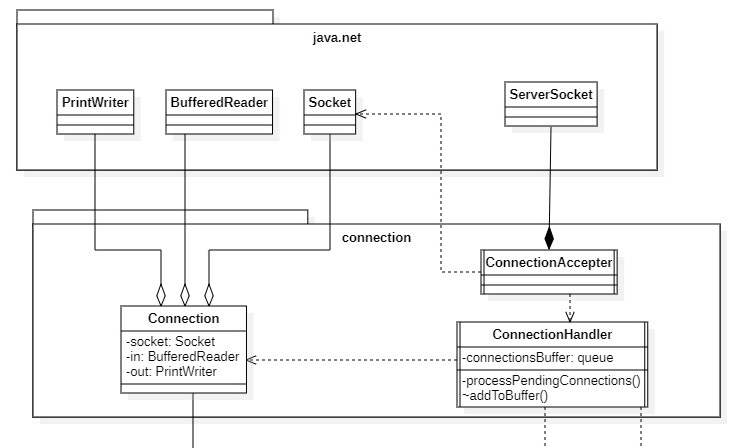
\includegraphics[scale=0.55]{res/diagrams/server/server_communication.jpg}
	\caption{Visione di dettaglio del Communication Layer}
\end{figure}


Questo layer si interfaccia con i client esterni e ha lo scopo di gestire la comunicazione con questi. In particolare, la classe \texttt{ConnectionAccepter} si occupa di accettare le nuove connessioni entranti tramite \texttt{ServerSocket}: essa esegue su un thread dedicato in modo da non bloccare le altre operazioni all'arrivo di una nuova connessione.

Per ogni nuova connessione, crea un oggetto \texttt{Socket} che passa a \texttt{ConnectionHandler}. Quest'ultima è una componente che esegue su un altro thread dedicato: rimane in attesa fino al risveglio determinato da \texttt{ConnectionAccepter}: una volta attivato, procede a svuotare il buffer di \texttt{Socket} per creare oggetti di tipo \texttt{Connection}, istanziando per ognuno i buffer di input e output. Segue quindi il processo di autenticazione dei muletti o degli utenti, al termine del quale \texttt{ConnectionHandler} torna in attesa.

    \pparagraph{Incrementare il livello di sicurezza}
    Essendo PORTACS\textsubscript{A} inserito in un contesto limitato al campo di operazione e non pubblico, gode di una sicurezza intrinseca essendo la rete privata e non esposta o accedibile all'esterno. Tuttavia all'interno della rete, le comunicazioni tra server e clients avvengono in chiaro. Se si vuole più sicurezza ci si può dotare di un certificato TLS\textsubscript{A} e sostituire l'implementazione di ServerSocket e Socket rispettivamente con SSLServerSocket e SSLSocket. Dopodiché si dovrà sostituire nella parte node dei client la libreria net con quella tls e configurare il certificato. Non saranno necessarie ulteriori variazioni. Maggiori informazioni:
    \begin{itemize}
        \item \href{https://docs.oracle.com/en/java/javase/15/docs/api/java.base/javax/net/ssl/SSLServerSocket.html}{SSLServerSocket};
        \item \href{https://docs.oracle.com/en/java/javase/15/docs/api/java.base/javax/net/ssl/SSLSocket.html}{SSLSocket};
        \item \href{https://blogs.oracle.com/blogbypuneeth/steps-to-create-a-self-signed-certificate-using-openssl}{blog oracle sui certificati};
        \item \href{https://nodejs.org/api/tls.html}{libreria TLS\textsubscript{A} per node}.
    \end{itemize}





\clearpage
\subsubsection{Business layer}

Nel Business layer risiede il nucleo di elaborazione dei dati ricevuti dal layer superiore: i domini principali di cui si occupa sono:
\begin{itemize}
	\item gestione della mappa e path finding;
	\item autenticazione dei client;
    \item elaborazione delle richieste;
	\item gestione delle tasks e dei POI\textsubscript{A};
	\item rilevazione e risoluzione delle collisioni.
\end{itemize}
Per facilitare la consultazione, lo studio di questo layer si concentra separatamente sui package di cui si compone. Per una visione dall'alto, riferirsi al diagramma complessivo all'inizio della sezione 5.1.



\clearpage
\pparagraph{Clients}

\begin{figure}[H]
	\centering
	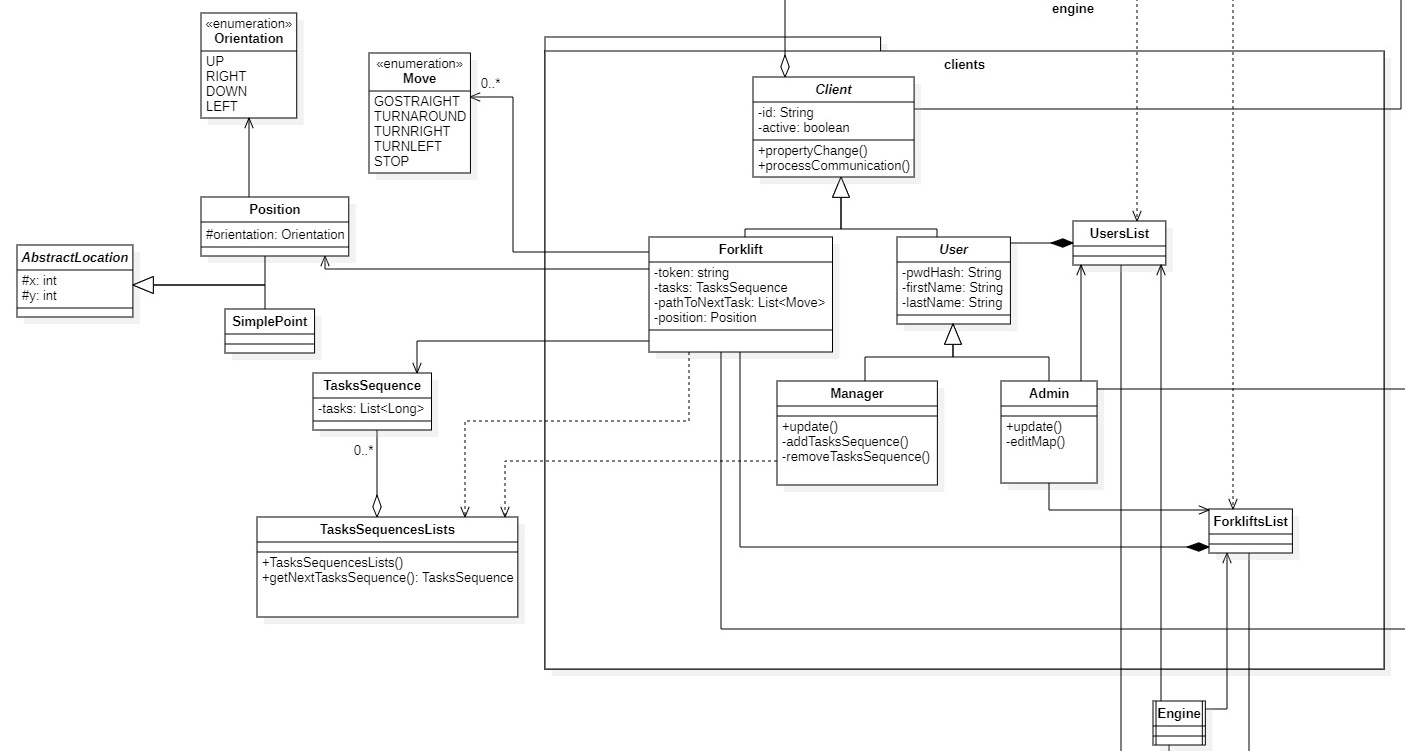
\includegraphics[scale=0.40]{res/diagrams/server/server_pack_clients.jpg}
	\caption{Visione di dettaglio del package Clients}
\end{figure}

La gerarchia dei \texttt{Client} prevede una prima suddivisione suddivisione tra \texttt{Forklift} e \texttt{User} (muletto e utente), gli \texttt{User} si specializzano ulteriormente in \texttt{Manager} (responsabile) e \texttt{Admin} (amministratore). Viene mantenuto a runtime lo stato di tutti i muletti e degli utenti registrati rispettivamente in \texttt{ForkliftsList} e \texttt{UsersList} così da ridurre le operazioni sulla persistenza.

I \texttt{Forklift} si caratterizzano dagli attributi:
\begin{itemize}
	\item \texttt{position}: rappresenta la posizione e orientamento attuali del muletto nella mappa;
	\item \texttt{tasks}: sequenza di task\textsubscript{G} da compiere;
	\item \texttt{pathToNextTask}: una lista di mosse atte a raggiungere il prossimo POI\textsubscript{A} (e quindi evadere la prossima task).
\end{itemize}

Notare che ogni \texttt{Client} possiede un attributo di tipo \texttt{Connection}, attraverso il quale viene regolata la comunicazione tramite Socket (per i dettagli si rimanda alle \S\ \ref{communication-layer} e \ref{communication-section}). Questo viene assegnato all'autenticazione e può cambiare un numero indefinito di volte, ogni qual volta che la connessione con il client verrà chiusa per qualsiasi ragione alla riconnessione questa verrà correttamente abbinata alla sua istanza.\\

La classe \texttt{Engine} è il cuore del motore di calcolo: essa esegue su un thread dedicato e tramite un timer scandisce l'esecuzione temporizzata dell'elaborazione. In particolare, interroga periodicamente \texttt{ForkliftsList} e \texttt{UsersList} con i seguenti obiettivi:
\begin{itemize}
	\item ricevere le nuove posizioni dai muletti;
	\item inviare le nuove informazioni agli utenti per la visualizzazione nel monitor real-time;
	\item rispondere ad eventuali altre richieste dell'iterazione precedente, avendo nel frattempo completato la loro elaborazione (calcolo percorso, aggiunta task\textsubscript{G}, modifica mappa).
\end{itemize}
Dopodichè la \texttt{ForkliftsList} viene utilizzata dal modulo di rilevazione e gestione delle collisioni.

In questo layer si concentra l'utilizzo del framework\textsubscript{G} Spring, utilizzato per gestire le dipendenze: alcune classi di utilizzo frequente e condiviso come \texttt{UsersList}, \texttt{ForkliftsList} e \texttt{TasksSequencesLists} (quest'ultima contenente tutte le liste di task\textsubscript{G} inserite dal responsabile) vengono istanziate tramite \textit{Dependency Injection} sfruttando il meccanismo dei \textit{Bean} di Spring.

    \ssubparagraph{Introdurre nuove tipologie di utenti}
        Per introdurre nuove tipologie di utenti, bisogna estendere la classe astratta User e concretizzare in classi concrete, erediterà i campi principali, si può aggiungere altri metodi e attributi, ma è necessario fare l'override del metodo ProcessComunication, che si occupa di gestire la comunicazione, in particolare ricevere i messagi, eseguire quello che viene richiesto e inviare i dati necessari.


\clearpage
\pparagraph{Mappa}

\begin{figure}[H]
	\centering
	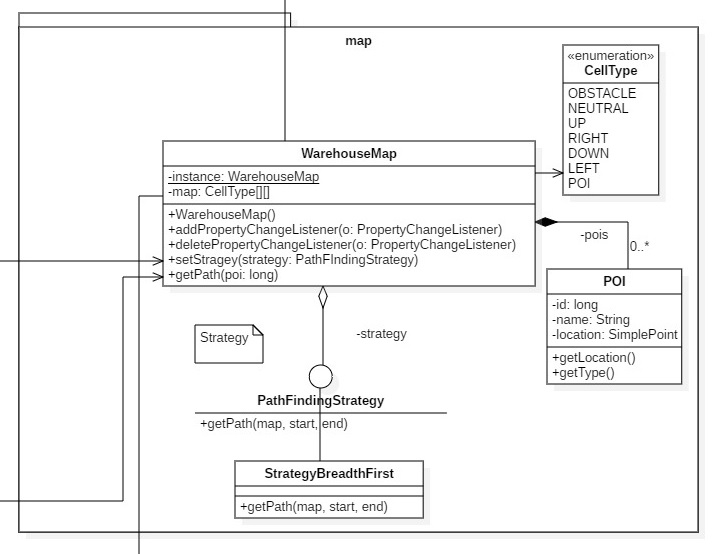
\includegraphics[scale=0.60]{res/diagrams/server/server_pack_map.jpg}
	\caption{Visione di dettaglio del package Map}
\end{figure}


La classe \texttt{WarehouseMap} contiene la rappresentazione della planimetria\textsubscript{G} del magazzino: essa è rappresentata tramite una matrice di \texttt{CellType}, campo di tipo enumerazione che esprime le caratteristiche di ogni frazione spaziale. Alla mappa è associata una lista di POI\textsubscript{A}, e per ognuno la relativa locazione.
Si osserva l'applicazione di alcuni design pattern\textsubscript{G}:
\begin{itemize}
	\item \textbf{observer}: tramite \texttt{PropertyChangeSupport} e \texttt{PropertyChangeListener} di \texttt{java.beans} viene applicato il pattern \textit{observer}, definendo la \texttt{WarehouseMap} come Subject, e i \texttt{Client} come \textit{Observer}: essi verranno notificati ad ogni cambiamento della stessa in modo che possano comunicarlo tramite le connessioni, così da riflettere le modifiche ed aggiornare le interfacce grafiche che visualizzano la mappa;
	\item \textbf{strategy}: per l’algoritmo di path finding attualmente viene implementata una strategia di tipo \textit{breadth-first}, ma l’impostazione del pattern permette di aggiungere e variare dinamicamente eventuali altre implementazioni aggiunte in futuro. \texttt{WarehouseMap} assume il ruolo di \textit{context}, e i beneficiari sono i \texttt{Forklift}, i quali richiederanno il percorso ogni qualvolta si renderà necessario.
\end{itemize}
\ssubparagraph{Estendere il path finding}
Si può aggiungere un algoritmo alternativo di path finding, oltre a quello già implementato con una strategia breadth first (in ampiezza).
Per farlo, bisogna creare una classe che implementi l'interfaccia \texttt{PathfindingStrategy}. Implementando questa interfaccia, viene creata una nuova strategia, e l'unica cosa necessaria da fare è implementare il metodo pubblico \texttt{getPath}, in quanto unico metodo utilizzato dall'esterno, che ritorna il percorso dal punto start a end sulla mappa, fatto di una list di moves (il nostro campo enum).
La strategia può essere cambiata tramite il metodo \texttt{setStrategy} nella classe \texttt{WareHouseMap} e dunque cambiare quella di default nella configurazione di Spring, oppure si può aggiungere un'operazione per l'amministratore per cambiare quella di default a run-time.




\clearpage
\pparagraph{Collisioni}
\label{collision-details}

\begin{figure}[H]
	\centering
	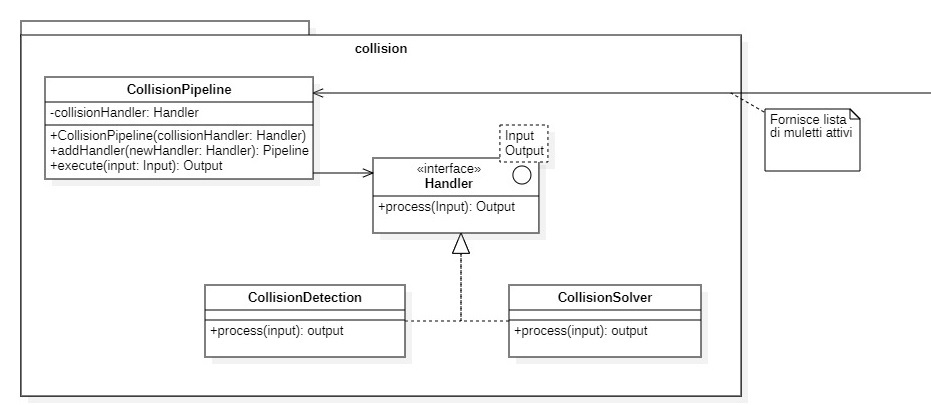
\includegraphics[scale=0.60]{res/diagrams/server/server_pack_collision.jpg}
	\caption{Visione di dettaglio del package Collision}
\end{figure}


Qui è contenuta la logica che gestisce le collisioni fra i muletti che circolano in guida autonoma all'interno del magazzino. L'elaborazione è scandita dal timer dell'\texttt{Engine}: ad ogni intervallo di tempo, vengono eseguite due operazioni sequenziali:
\begin{itemize}
	\item \textbf {rilevazione degli stalli:} vengono individuate le unità che rimangono in stallo per un tempo superiore ad una soglia prestabilita, sintomo di una condizione critica nella circolazione dei muletti. La componente \texttt{DeadlockCheck} si occupa di gestire queste situazioni;
	\item \textbf{rilevazione delle collisioni:} conoscendo le future mosse di ogni unità, vengono determinate le possibili collisioni tra le stesse. La componente \texttt{CollisionDetection} esegue queste operazioni;
	\item \textbf{gestione collisioni frontali:} sulla base delle collisioni eventualmente rilevate, vengono gestite le potenziali collisioni frontali, che richiedono una risoluzione particolare. Questo step è svolto dalla componente \texttt{HeadOnCollisions};
	\item \textbf{gestione delle precedenze:} l'ultimo passo risponde all'esigenza di stabilire delle precedenze durante la normale circolazione dei muletti: sulla base delle potenziali collisioni rilevate, alcuni si fermeranno per lasciare passare gli altri. Di ciò si occupa la componente \texttt{NearestToCollision}.
\end{itemize}


Viene applicato in questo contesto il design pattern\textsubscript{G} \texttt{Pipeline}\footnote{Variante del pattern \textit{Chain Of Responsibility}: \url{https://java-design-patterns.com/patterns/pipeline/}}, che permette di definire vari \texttt{Handler} da comporre come catena di operazioni. La pipeline può essere poi eseguita (se necessario, come in questo caso, ripetutamente) con un comando che attiva i vari step sequenzialmente. Ogni \texttt{Handler} specifica i tipi del proprio parametro di input e di output: l'output di un \texttt{Handler} sarà l'input dell'\texttt{Handler} successivo.
In questo caso l'input sarà una struttura rappresentante muletti attivi con le loro posizioni e prossime mosse, mentre l'output un'altra struttura che ad ogni punto con collisione associ i muletti coinvolti e le azioni da intraprendere così da poterle comunicare.

    \ssubparagraph{Modificare handler per la gestione delle collisioni}
        La struttura fornita dal design pattern\textsubscript{G} \textit{Pipeline}, come anticipato nella \S \ref{collision-details}, consente di concatenare operazioni da eseguirsi sequenzialmente e il cui output di ognuna costituisce l'input della successiva. Per aggiungere un'operazione è necessario implementare l'interfaccia \texttt{Handler<I,O>} specificando i parametri di input (\texttt{I}) e di output (\texttt{O}) del nuovo \texttt{ConcreteHandler}. La logica dell'operazione si costruisce eseguendo l'\textit{Override} del metodo \texttt{Process(I input) : O}. La costruzione della pipeline prevederà l'aggiunta del nuovo \texttt{ConcreteHandler} tramite il metodo \texttt{addHandler} in modo che l'esecuzione, avviata invocando il metodo \texttt{execute}, includa la nuova operazione nella sua sequenza.

        L'applicazione di questo design pattern\textsubscript{G} consente di modificare facilmente le operazioni che compongono la sequenza: se necessario, è possibile sostituirle anche tutte, cambiando di fatto l'implementazione dell'algoritmo; mantenendo però intatti i parametri di ingresso e uscita.



\subsubsection{Persistence layer}

\begin{figure}[H]
	\centering
	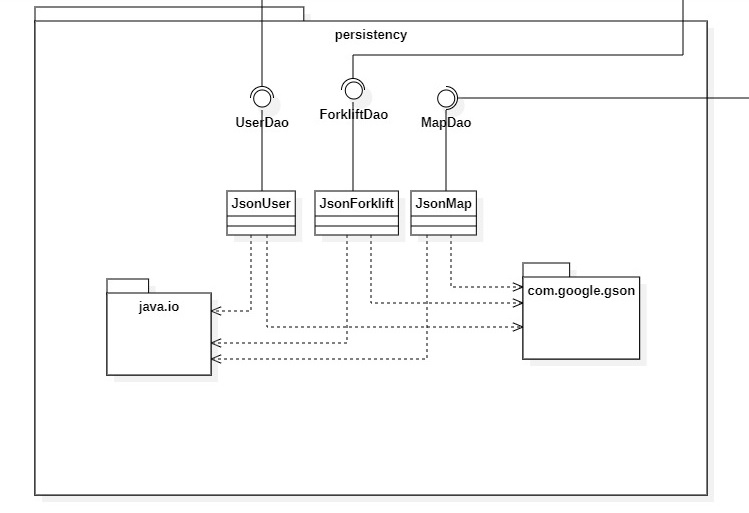
\includegraphics[scale=0.50]{res/diagrams/server/server_persistency.jpg}
	\caption{Visione di dettaglio del Persistence Layer}
\end{figure}

L'accesso a questo layer è regolato da 3 interfacce che gestiscono la persistenza delle tre tipologie di dati che vengono salvati:
\begin{itemize}
	\item i dati e le credenziali degli utenti;
	\item gli identificativi ed i token di autenticazione dei muletti;
	\item la rappresentazione della mappa.
\end{itemize}

Ogni interfaccia si rivolge alla relativa componente del layer superiore che conserva a runtime i dati impiegati nell'esecuzione. La presenza delle interfacce favorisce il disaccoppiamento tra i moduli e permette di estendere a tipi di persistenza alternativi. Attualmente è implementato il salvataggio dei dati su file di tipo .json, viene fatto uso della libreria standard java.io e GSON per gestire l'interazione con questo tipo di tecnologia.

    \pparagraph{Implementare tipi di persistenza alternativi}
        Le interfacce \texttt{UserDao}, \texttt{ForklistDao} e \texttt{MapDao} forniscono i contratti sulla persistenza di utenti, muletti e mappa. Per implementare un nuovo tipo di persistenza bisogna creare una classe, implementando una di questa 3 interfacce, in base alla tipologia, e implementare i metodi richiesti dall'interfaccia.
        Similmente all'algoritmo di \texttt{pathfinding}, per settare questo tipo di persistenza bisogna passare per la configurazione Spring, per la gestione delle \textit{dependency injection}.


\pagebreak
